% !TeX root = ../../tesis.tex

% -----------------------------------------------------------------------
\subsection{Nivel de Alimentación Capilar --- Fuerza Nodal \texorpdfstring{($C_i$)}{(Ci)}}
\label{subsec:alimentacion-capilar}
% -----------------------------------------------------------------------

\textbf{Fuente principal:} \citet{lee2008}

\subsubsection{Definición y Fundamentación}

Una vez que las estaciones están georreferenciadas y las aristas de la red están
conectadas, el siguiente paso es identificar el rol funcional de cada nodo en la
jerarquía del sistema. \citet{lee2008}, en su análisis estadístico de la red de
metro de Seúl, establecen que cada estación puede caracterizarse por dos
propiedades complementarias: su \termino{grado} ($k$), definido como el número
de conexiones (aristas) que entran o salen del nodo, y su \termino{fuerza}
($s$), definida como la suma de los pesos (flujos de pasajeros) de todos los
enlaces conectados a esa estación.

Los autores demuestran que la distribución de la fuerza de los nodos en la red
de metro de Seúl sigue un comportamiento log-normal con un pico característico,
lo que indica que la mayoría de las estaciones atienden un volumen similar de
pasajeros, pero un pequeño número de nodos ---los grandes concentradores o
\textit{hubs}--- acumula flujos desproporcionadamente elevados. Este patrón es
directamente relevante para la red de la \cdmx{}, donde los macro-CETRAMs
(Pantitlán, Indios Verdes, Cuatro Caminos, Taxqueña) operan como \textit{hubs}
nodales que concentran la articulación entre las redes capilares de superficie y
las arterias masivas.

\subsubsection{Fórmula}

\begin{equation}
    C_i = \sum_{j \in S} A_{ij} \cdot \peso{i}{j}
    \label{eq:fuerza-nodal}
\end{equation}

Donde:
\begin{itemize}
    \item $C_i$ = Nivel de Alimentación Capilar (Fuerza Nodal) de la estación
    masiva $i$.
    \item $S$ = Subconjunto de rutas pertenecientes exclusivamente a la red de
    superficie (RTP, microbús, trolebús, concesionados).
\item $A_{ij}$ = Elemento de la matriz de adyacencia: 1 si la ruta de superficie
    $j$ conecta con la estación masiva $i$, 0 en caso contrario.
\item $\peso{i}{j}$ = Peso de la conexión: capacidad de pasajeros por hora o
flujo
    real medido de la ruta $j$ en la estación $i$.
\end{itemize}


\citet{lee2008} establecen que el peso $\peso{i}{j}$ de un enlace representa el
flujo de pasajeros que transita por él, y que la fuerza $s_i$ de una estación
corresponde al número de pasajeros que llegan y parten de ella. En el modelo
propuesto, $\peso{i}{j}$ se inicializa con la capacidad operativa declarada de
cada ruta y se refinará en fases posteriores con el Coeficiente de Fricción
Vial.

\begin{figure}[H]
    \centering
    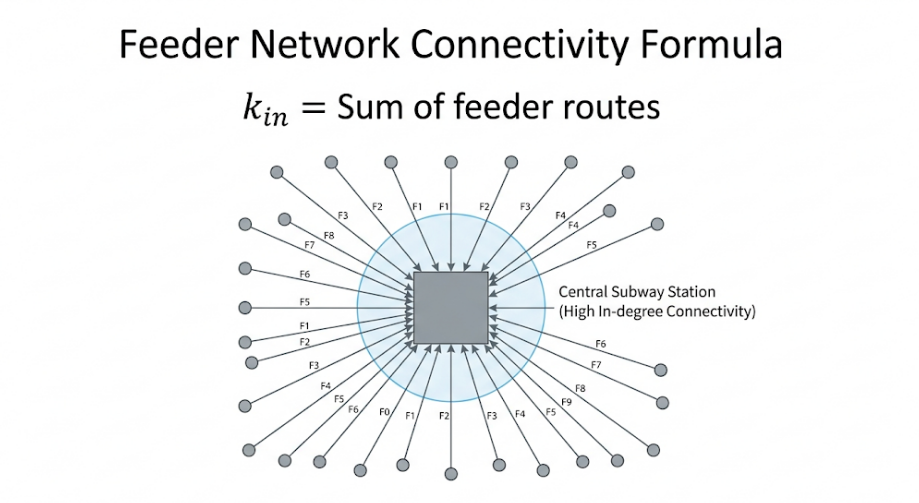
\includegraphics[width=0.70\textwidth]{Figures/Cap3/NiveldeAlimentacionCapilar.png}
    \caption[Diagrama del indicador de Alimentación Capilar $C_i$]{Esquema de
    fuerza nodal: rutas de superficie $F_1 \ldots F_n$ convergiendo en una
    estación masiva de alta conectividad de entrada.}
    \label{fig:indicador-Ci}
    \fuentefigura{Elaboración propia con base en \citet{lee2008}.}
 \end{figure}


\subsubsection{Ejemplo Práctico: \cdmx{} y Zona Metropolitana}

\begin{table}[H]
    \centering
    \caption{Estimaciones del indicador $C_i$ en nodos representativos.}
    \label{tab:capilar-nodos}
    \begin{tabularx}{\textwidth}{X r r}
        \toprule
        \textbf{Estación masiva} &
        \textbf{$k_{in}$ (rutas capilares)} &
        \textbf{$C_i$ estimado (pax/h)} \\
        \midrule
        Pantitlán (Hub CETRAM)          & $\approx 120$ rutas & Alto \\
        Indios Verdes (CETRAM)          & $\approx 90$ rutas  & Alto \\
        Nodo Norte propuesto (Periférico) & $\approx 40$ rutas (est.) & Medio-alto \\
        \bottomrule
    \end{tabularx}
\end{table}

La implementación computacional de referencia para este indicador se encuentra
en el \autoref{anx:indicadores-implementacion} (§\ref{anx:impl-capilar}).

La fuerza nodal $C_i$ complementa al indicador $C$ en la consecución del
Objetivo Específico 4 (§\ref{subsec:obj-especificos}): mientras $C$ mide el
alcance territorial de la red, $C_i$ cuantifica la intensidad de la articulación
capilar en cada nodo masivo, identificando cuáles de ellos concentran mayor
presión de demanda y constituyen, por tanto, los candidatos prioritarios para la
ampliación de la red con corredores perimetrales.
